\chapter{QUADRO TEÓRICO}

	\par Neste capítulo serão descritos os principais conceitos e características
das tecnologias utilizadas para o desenvolvimento dos \textit{softwares}
propostos nos objetivos deste trabalho.

\section{\textit{Java}}

	\par Segundo \citeonline{deitel2002} o \textit{java} veio ao público em 1995 pela
\textit{Sun Microsystem}. Os criadores dessa nova tecnologia liderados por
James Gosling basearam-se em duas linguagens muito utilizadas no mundo, C e C++.
Isso deu ao java uma base para implementar em novos sistemas como, sistemas
operacionais, sistemas de comunicações, sistema de banco de dados e aplicativos
para computadores pessoais.

	\par Entre as principais características pode-se dizer que o Java é:
	
	\begin{itemize}

	  \item Orientado a objeto.
	  
	  \item Seguro.%explicar um pouco melhor
	  
	  \item Independente de plataforma. 

	\end{itemize}
	
	\par \citeonline{deitel2002} o \textit{java} será utilizado para codificar e
criar regras para proteger o banco de dados, gerenciando a infraestrutura que
o próprio java fornece como, Transação, Acesso remoto, Web services,
Gerenciamento de threads, Gerenciamento de conexões http\footnote{HTTP -
HyperText Transfer Protocol.}.

	\par Para acessar o servidor precisamos de um serviço \textit{web} (\textit{Web
services}) que utilizará o \textit{java} para criar as regras e serviços de
compilação de dados. Segundo \citeonline{deitel2002} existem cinco fases para
que os dados cheguem em seu dispositivo que são, armazenamento em disco, o
compilador cria os \textit{bytecodes}, transfere-os para memória, verifica a sua
integridade, para que não haja nenhuma violação das restrições de segurança e
por ultimo o interpretador(JMV\footnote{JVM - Java Virtual Machine}) lê os
\textit{bytecodes} e os traduz para a linguagem que o computador entenda e
possivelmente armazena os valores dos dados enquanto executa o programa.

	\par \citeonline{romanato2015} afirma que o \textit{Java} usa a JMV, que é
uma máquina virtual capaz de converter os \textit{bytecodes} para a linguagem
do sistema operacional utilizado pelo cliente, sem a necessidade de compilá-lo
para cada plataforma. Dessa maneira um \textit{software} que foi desenvolvido
para um sistema operacional, funcionará normalmente em qualquer outro.

\section{\textit{Android}}

	\par Segundo \citeonline{monteiro2012}, \textit{Android} é um sistema
operacional baseado em \textit{Linux}, de código aberto e que utiliza a
linguagem de programação \textit{Java} para o desenvolvimento de seus
aplicativos. Criado especialmente para dispositivos móveis, começou a
ser desenvolvido no ano de 2003 pela então empresa Android Inc, que em 2005 foi
agregada ao Google. A partir de 2007 o projeto \textit{Android} uniu-se a
\textit{Open Handset Alliance}, uma associação de empresas de
\textit{softwares}, \textit{hardwares} e telecomunicações, que tem por
finalidade desenvolver uma plataforma para dispositivos móveis que seja
completa, aberta e gratuita.

	\par \citeonline{krazit2009} publicou uma entrevista com Rubin, um dos
idealizadores do \textit{Android}, o qual afirma que o sistema pode rodar em
equipamentos de diversos fabricantes, evitando assim ficar limitado a poucos
dispositivos. Conforme informações do site \citeonline{android1}, hoje em dia
existe mais de um bilhão de aparelhos espalhados pelo mundo com esse sistema
operacional.

	\par De acordo com \citeonline{monteiro2012}, as aplicações são executadas em
uma máquina virtual Java denominada \textit{Dalvik}. Cada aplicativo, usa uma
instância dessa máquina virtual tornando-o assim mais seguro. Por outro lado, os
\textit{softwares} só podem acessar os recursos do dispositivo, como uma
lista de contatos, caso seja formalmente aceito pelo usuário nos termos de uso
ao instalá-lo.

	\par As configurações de uma aplicação na plataforma \textit{Android} ficam
salvas em um arquivo XML denominado AndroidManifest.xml que se localiza na raiz
do projeto. Para \citeonline{lecheta2010} as informações devem estar entre tags
correspondentes ao recurso. De forma, que o arquivo se inicie pela tag
<manifest> e se encerre por </manifest>. Com necessidade de acessar a internet
é preciso declarar a permissão da seguinte forma <uses-permission
android:name="android.permission.internet" />.

	\par \citeonline{lecheta2010} diz que as \textit{intents} podem ser
consideradas como o coração do \textit{Android}, uma vez que essa classe está
presente em todos os lugares de uma aplicação. De acordo com
\citeonline[p.29]{k192012}, "são objetos responsáveis por passar informações,
como se fossem mensagens, para os principais componentes da API do
\textit{Android}, como as \textit{Activities}, \textit{Services} e
\textit{BroadCast Receivers}". \citeonline{monteiro2012} diz que as
\textit{Intents} são criadas quando se tem a intenção de realizar algo como por
exemplo compartilhar uma imagem, utilizando os recursos já existentes no
dispositivo. Existem dois tipos de Intents:
	
	\begin{itemize}
	  
	  \item \textit{Intents} implícitas - Quando não é informada qual
	  \textit{Activity} deve ser chamada, ficando assim por conta do sistema
	  operacional verificar qual a melhor opção.
	  
	  \item \textit{Intents} explicitas - Quando é informada qual
	  \textit{Activity} deve ser chamada. Usada normalmente para chamar
	  \textit{activities} da mesma aplicação.
	  
	\end{itemize}
	
	\par Segundo \citeonline{k192012}, uma aplicação \textit{Android} pode ser
construída com quatro tipos de componentes: \textit{Activity},
\textit{Services}, \textit{Content Providers} e \textit{Broadcast Receivers}.

	\par As \textit{activities} são as telas com interface gráfica, que permitem
interações com os usuários. De acordo com \citeonline{lacheta2013}, cada
\textit{activity} tem um ciclo de vida, uma vez que ela pode estar sendo
executada, estar em segundo plano ou totalmente destruída.

	\par Toda vez que é iniciada uma \textit{activity}, ela vai para o topo de uma
pilha denominada \textit{activity stack}. O bom entendimento do ciclo de vida é
importante, pois quando uma aplicação é interrompida é possível salvar as
informações ou ao menos voltar ao estágio a qual o usuário se encontrava. Na
Figura \ref{fig:qt1} é demostrado um exemplo de ciclo de vida de uma
\textit{activity}.

\begin{figure}[h!]
	\centerline{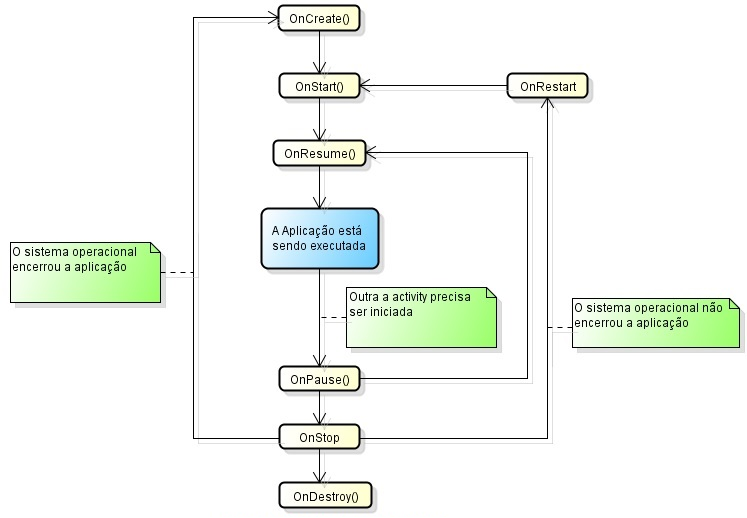
\includegraphics[scale=0.5]{./imagens/1_q_teorico/qt1.png}}
	\caption[Ciclo de Vida de uma \textit{Activity} ]{Ciclo de Vida de uma
	\textit{Activity}.
	 \textbf{Fonte:}\citeonline{lecheta2010}}
	\label{fig:qt1}
\end{figure}

	\par Para que se possa entender melhor imagina- se o
seguinte cenário: Um usuário entra no aplicativo de notas da Univás. Para que a
\textit{activity} seja criada é chamado o método \textit{OnCreate()}, logo após
é executado o método \textit{OnStart()} e ao finalizar do ciclo anterior é
chamado o \textit{OnResume()}, só a partir de então, a \textit{activity} é
visualizada pelo usuário. Contudo, durante a navegação o aluno recebe uma
ligação. Nessa hora o sistema operacional chama o método \textit{OnPause()}
para pausar a aplicação e abrir uma outra \textit{activity} para que o usuário
possa atender a chamada telefônica. É possível nesse método salvar informação
da qual o usuário está utilizando. Ao concluir o método de pausa é executado o
método \textit{OnStop()}, a partir de agora a \textit{activity} da Univás não
será mais visível para o usuário. Ao encerrar a ligação, há dois caminhos
possíveis de se percorrer, o primeiro, é o caso do sistema operacional não
encerrar completamente a aplicação da memória, dessa forma será chamado o
método \textit{OnRestart()} do aplicativo de notas e voltar de onde o usuário
estava, porém se foi necessário encerrar completamente a aplicação, devido à
falta de memória, será necessário chamar o método \textit{OnCreate()}
novamente. Por fim quando o usuário sair da aplicação é chamado o método
\textit{OnDestroy()} encerrando se assim o ciclo de vida.

	\par No arquivo AndroidManifest.xml as \textit{activities} devem estar entre as
tags \textit{<activity> </activity>} e a \textit{activity} principal, ou seja,
pela qual será iniciada a aplicação deve conter a tag <\textit{intente-filter}>
além de <\textit{action android:name="android.intent.action.MAIN"}/> indicando
que essa atividade deverá ser chamada ao iniciar a aplicação e\linebreak[4]
<\textit{category android:name="android.intent.category.LAUNCHER"}/> que
implica que esse APP ficará disponível junto aos outros aplicativos no
dispositivo.

	\par A \textit{Activity} a ser utilizada para iniciar a aplicação é uma
\textit{Navigation Drawer}. Segundo o site \citeonline{android2015} ela exibe
do lado esquerdo as principais funções do \textit{software}, semelhante a um
menu. Fica normalmente escondida aparecendo apenas quando se clica no canto
superior esquerdo.

	\par Segundo \citeonline{lecheta2010}, a classe \textit{Services} existe
com intuito em executar processos que levarão um tempo indeterminado para serem
executados e que normalmente consomem um alto nível de memória e processamento.
Esses processos são executadas em segundo plano enquanto o cliente realiza
outra tarefa. Assim um usuário pode navegar na internet enquanto é feito um
\textit{download}. O serviço é geralmente iniciado pelo \textit{Broadcast
Receiver} e quem o gerencia é o sistema operacional que só o finalizará ao
concluir a tarefa, salvo quando o espaço de memória é muito baixo.

	\par Para \citeonline{lecheta2010}, a função da classe \textit{Content
Provider} é prover conteúdos de forma pública para todas as aplicações, dessa
forma usando-se essa classe é possível as aplicações consultar, salvar, deletar
e alterar informações no \textit{smartphone}. Assim afirma
\citeonline[p.413]{lecheta2010} “O \textit{Android} tem uma série de provedores
de conteúdo nativos, como, por exemplo, consultar contatos da agenda,
visualizar os arquivos, imagens e vídeos disponíveis no celular”. Portanto, um
contato pode ser salvo por um aplicativo e alterado por outro.

	\par Para \citeonline{lecheta2010}, a classe \textit{Broadcast Receiver}
é muito importante para a plataforma \textit{Android}, uma vez que ela é
responsável por agir em determinados eventos de uma \textit{intent}.

	\par Essa classe sempre é executada em segundo plano, de forma que o usuário
não veja o que está sendo executado. Portanto, quando uma pessoa está
utilizando uma aplicação e recebe uma mensagem de SMS, o \textit{Broadcast
Receiver} capta essa informação e a processa sem a necessidade do cliente ter
que parar de realizar suas tarefas.

	\par A configuração de um \textit{Broadcast Receiver} é escrita pela tag
<\textit{receiver}> junto com a tag <\textit{intente-filter}> que conterá o que
deve ser feito dentro do AndroidManifest.xml.

	\par Em uma aplicação, um elemento fundamental é a interface gráfica, que
deverá ser organizada, simples e elegante. Conforme \citeonline{monteiro2012}
esses são os principais \textit{Layouts} do sistema operacional Android:
	\begin{itemize}
	
	 \item \textit{LinearLayout} - Permite posicionar os elementos em forma
	 linear, dessa forma quando o dispositivo estiver em forma vertical os itens
	 ficaram um abaixo do outro e quando estiver na posição horizontal eles
	 ficaram um ao lado do outro.
	
	  \item \textit{RelativeLayout} - Permite posicionar elementos de forma
	  relativa, ou seja um item com relação a outro.
	
	  \item \textit{TableLayout} - Permite criar \textit{layouts} em formato de
	  tabelas. O elemento \textit{TableRow} representa uma linha da tabela e seus
	  filhos as células.  Dessa maneira, caso um \textit{TableRow} possua dois
	  itens significa que essa linha tem duas colunas.
	
	  \item \textit{DatePicker} - \textit{Widget} desenvolvido para a seleção de
	  datas que podem ser usadas diretamente no \textit{layout} ou através de
	  caixas de diálogo.

	  \item \textit{Spinner} - \textit{Widget} que permite a seleção de itens. 
	
	  \item \textit{ListViews} - Permite exibir itens em uma listagem. Dessa
	  forma, em uma lista de compras, clicando em uma venda é possível listar os
	  itens dessa venda selecionada.
	
	  \item \textit{Menus} - Um item muito importante, pois apresenta aos usuários
	  as opções existentes no aplicativo.
	
	  \item \textit{AlertDialog} - Apresenta informações aos usuários através de
	  uma caixa de diálogo. Comumente utilizado para perguntar ao cliente o que
	  deseja fazer quando seleciona algum elemento.
	
	  \item \textit{ProgressDialog} e \textit{ProgressBar} - Utilizado quando uma
	  aplicação necessita de um recurso que será demorado, como por exemplo, fazer
	  um \textit{download}, pode ser feito uma animação informando ao usuário o
	  progresso da operação.
	
	\end{itemize}
	
	\par Para uma maior interação, as aplicações normalmente utilizam API’s de
terceiros, como o Google \textit{Maps}, quando necessita encontrar alguma
localização. Para \citeonline{monteiro2012} essa comunicação pode utilizar o
REST\footnote{REST - \textit{Representational State Transfer} ou Transferência
de Estado Representativo.}, que envia requisições através da URL. Ao receber
informações pedidas a um outro serviço, ela pode estar no padrão XML ou JSON. O
REST será detalhado mais adiante.

	\par Outra ferramenta importante e muito utilizada do Android é a Notificação.
Segundo \citeonline{phillips2013}, quando uma aplicação está sendo executada em
segundo plano e necessita comunicar-se com o usuário, o aplicativo cria uma
notificação. Normalmente as notificações aparecem na barra superior, o qual
pode ser acessado arrastando para baixo a partir da parte superior da tela.
Assim que o usuário clica na notificação ela cria uma \textit{activity} abrindo
a aplicação em questão.

	\par Com a ideia de desenvolver um aplicativo para dispositivos móveis, a
plataforma Android foi escolhida devido ao seu destaque no mercado e pela
facilidade que apresenta aos usuários.

\section{Android Studio}

	\par Umas das ferramentas mais utilizadas para o desenvolvimento em Android é o
\textit{Eclipse IDE}, contudo a Google criou um \textit{software} especialmente
para esse ambiente, chamado \textit{Android Studio}. Segundo
\citeonline{gusmao2014}, \textit{Android Studio} é uma IDE baseado no ItelliJ
\textit{Idea} e foi apresentado na conferência para desenvolvedores I/O de 2013.

	\par De acordo com \citeonline{hohensee2013}, o \textit{Android Studio} tem um
sistema de construção baseado em \textit{Gradle}, que permite aplicar
diferentes configurações no código quando há necessidade de criar mais de uma
versão, como por exemplo, um \textit{software} que terá uma versão gratuita e
outra paga, melhorando a reutilização do código. Com o \textit{Gradle} também é
possível fazer os \textit{downloads} de todas as dependências de uma forma
automática sem a necessidade de importar bibliotecas.

	\par \citeonline{hohensee2013} afirma que o \textit{Android Studio} é um editor
de código poderoso, pois tem como característica a edição inteligente, pois ao
digitar já completa as palavras reservadas do sistema operacional e fornece uma
organização do código mais legível.

	\par Segundo \citeonline{android2}, a IDE tem suporte para a edição de
interface, o que possibilita ao desenvolvedor arrastar os componentes que
deseja. Ao testar o aplicativo permite o monitoramento do consumo de memória e
de processador por parte do utilitário.

	\par \citeonline{gusmao2014} diz que a plataforma tem uma ótima integração com
o \textit{GitHub} e está disponível para \textit{Windows}, \textit{Mac} e
\textit{Linux}. Além disso os programadores terão disponíveis uma versão
estável e mais três versões que estarão em teste chamadas de \textit{Beta},
\textit{Dev} e \textit{Canary}.

	\par Devido ao \textit{Android Studio} ser uma ferramenta de fácil usabilidade
e a IDE oficial para o desenvolvimento Android, esta foi escolhida como ambiente de
construção do aplicativo.	
	
\section{\textit{Web Services}}
	
	\par Nos tempos atuais, com o grande fluxo de informação que percorre pelas
redes da \textit{internet} é necessário um nível muito alto de integração entre
as diversas plataformas, tecnologias e sistemas. Como uma provável solução para
esse ponto, já existem as tecnologias de sistemas distribuídos. Porém essas
tecnologias sofrem demasiadamente com o alto acoplamento de seus componentes e
também com a grande dependência de uma plataforma para que possam funcionar. Com
intuito de solucionar a estes problemas e proporcionar alta transparência entre
as várias plataformas, foram criados as tecnologias \textit{web services}.
	
	
	\par De acordo com \citeonline{erl2015}:
	\begin{citacao}
		No ano de 2000, a W3C (\textit{World Wide Web Consortium}) aceitou a submissão
		do \textit{Simple Object Access Protocol} (SOAP). Este formato de mensagem
		baseado em XML estabeleceu uma estrutura de transmissão para comunicação entre
		aplicações (ou entre serviços) via HTTP. Sendo uma tecnologia não amarrada a
		fornecedor, o SOAP disponibilizou uma alternativa atrativa em relação aos
		protocolos proprietários tradicionais, tais como CORBA e DCOM.
	\end{citacao}
	
	\par Considera-se então a existência dos \textit{web services} a partir daí. De
acordo com \citeonline{duraes2005}, \textit{Web Service} é um componente que
tem por finalidade integrar serviços distintos. O que faz com que ele se torne
melhor que seus concorrentes é a padronização do XML (\textit{Extensible Markup
Language}) para as trocas de informações. A aplicação consegue conversar com o
servidor através do  WSDL que é documento que contém as regras de
funcionamento do \textit{web service}.
	
	\par Segundo \citeonline{coulouris2013}, “Um serviço \textit{Web} (\textit{Web
service}) fornece uma interface de serviço que permite aos clientes interagirem
com servidores de uma maneira mais geral do que acontece com os navegadores
\textit{Web}”. Ainda de acordo com \citeonline{coulouris2013} os clientes (que
podem ser desde um navegador até mesmo outro sistema) acessam serviços 
\textit{Web} fazendo uso de requisições e respostas formatadas em XML e sendo
transmitidos pelo uso do protocolo HTTP. O uso dessas tecnologias tende a
facilitar acomunicação entre as diversas plataformas, e atende de uma forma
melhor que as técnologias já existentes. Porém, para que haja uma interação
transparente e eficaz, entre as diversas plataformas, é necessário uma
infraestrutura um pouco mais complexa para integrar todas essas tecnologias.
Essa infraestrutura é composta pelas tecnologias já citadas e por outros
componentes essenciais para disponibilização de serviços \textit{web}, como
mostra a Figura \ref{fig:qt2}.

\begin{figure}[h!]
	\centerline{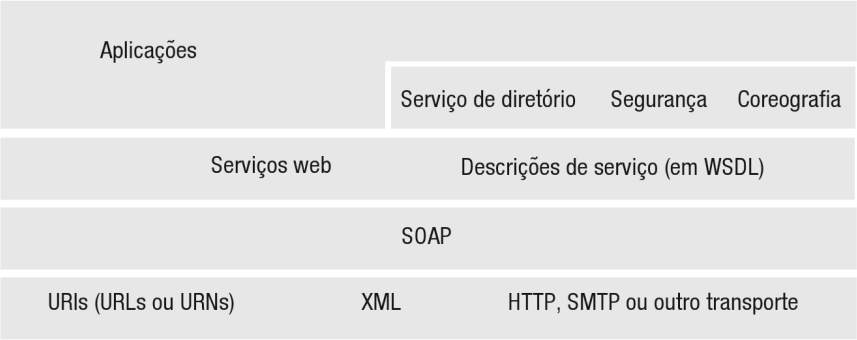
\includegraphics[scale=0.6]{./imagens/1_q_teorico/qt2.png}}
	\caption[Infraestrutura e componentes dos serviços
		\textit{web}. ]{Infraestrutura e componentes dos serviços
		\textit{web}. \textbf{Fonte:}\citeonline{coulouris2013}}
	\label{fig:qt2}
\end{figure}
	
	\par Os \textit{web services} geralmente fazem uso do protocolo SOAP, para
estruturar e encapsular as mensagens trocadas. De acordo com
\citeonline[p.381]{coulouris2013}, "O protocolo SOAP(\textit{Simple Object Access
Protocol}) é projetado para permitir tanto interação cliente-servidor como
assíncrona pela \textit{Internet}". Segundo \citeonline[p.27]{sampaio2006}, "O
SOAP foi criado inicialmente, para possibilitar a invocação remota de métodos
através da internet". As mensagens SOAP possuem um elemento Envelope. De acordo
com \citeonline[p.19]{saudate2013}, "O elemento Envelope é puramente um
\textit{container} para os elementos \textit{Header} e \textit{Body}". Ainda de
acordo com \citeonline{saudate2013}, o elemento \textit{header} transporta
metadados relativos à requisição tais como autenticação, endereço de retorno da
mensagem, etc. Já o elemento \textit{body} carrega o corpo da requisição, que
nada mais é do que o nome da operação e paramêtro referentes à mesma. É valido
que todas requisições do trocadas usando SOAP usam o XML com formato oficial. Na
Figura \ref{fig:qt3} está representado o esquema do Envelope SOAP.

\begin{figure}[h!]
	\centerline{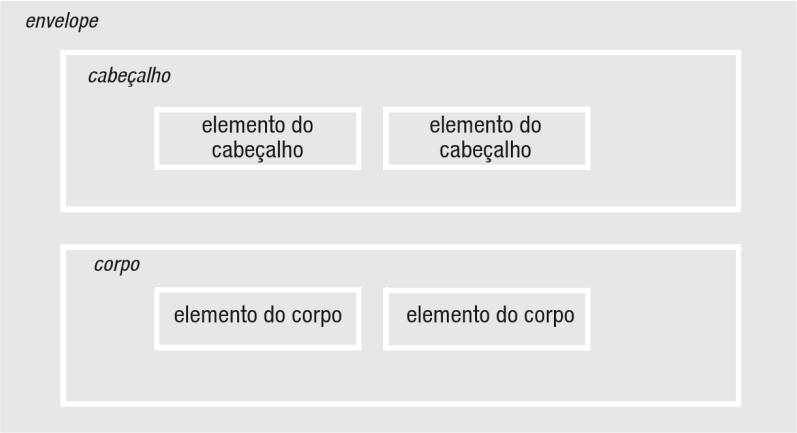
\includegraphics[scale=0.6]{./imagens/1_q_teorico/qt3.png}}
	\caption[Esquema de envelope SOAP. ]{Esquema de envelope SOAP. 
	 \textbf{Fonte:}\citeonline{coulouris2013}}
	\label{fig:qt3}
\end{figure}

	\par Os \textit{web services} além de fornecerem uma padronização de
comunicação entre as várias tecnologias existentes, provêem transparência na
troca de informações. Isso contribui pelo fato de que as novas aplicações
possam se comunicar com aplicações mais antigas ou aplicações contruídas sobre
outras plataformas.

	\par Além das tecnologias \textit{web services} tradicionais, existe também os
\textit{web services} REST que também disponibilizam serviços, porém não
necessitam de encapsulamento de suas mensagens assim como os \textit{web
Services} SOAP. Este fato influencia diretamente na performance da aplicação
como um todo, haja vista que não sendo necessário o encapsulamento da informação
requisitada ao \textit{web service}, somente é necessário o processamento e
tráfego da informação que realmente importa. As caracteristícas do padrão REST
serão abordadas a seguir.

	\subsection{REST}
	
	\par Segundo \citeonline{saudate2012}, REST é a sigla de
\textit{Representational State Transfer}, desenvolvido por Roy Fielding na
defesa de sua tese de doutorado. Segundo o próprio \citeonline{fielding2000}
REST é um estilo que deriva do vários estilos arquitetónicos baseados em rede
e  que combinado com algumas restrições, fornecem uma interface simples e
uniforme para fornecimento de serviços\footnote{Tradução e resumo de
informações de responsabilidade dos autores da pesquisa.}.
	
	\par \citeonline{rubbo2015} afirma que os dados e funcionalidade de um sistema
são considerados recursos e podem ser acessados através das URI's
\textit{(Universal Resource Identifier)}, facilitando dessa forma a comunicação
do servidor com o cliente. Um serviço baseado na arquitetura REST
basea-se fortemente em recursos. Para exemplificar o que seria um recurso em
REST têm-se o seguinte cenário: considera-se uma URL tal como 
http://www.univas.edu.br/alunos/ onde pretende-se fazer a gerência dos dados
de um ou de um conjunto de alunos. A recuperação de dados, bem como sua edição
e/ou deleção fazendo uso pleno dos métodos HTTP, através dessa URL pode ser
considerado como um recurso.
	\par \citeonline{saudate2012}, explica ainda que os métodos do HTTP podem fazer
modificações nos recursos, da seguinte forma:
	
	 \begin{itemize}
	   \item GET – Para recuperar algum dado. 
	   \item POST – Para criar algum dado.
	   \item PUT – Para alterar algum dado. 
	   \item DELETE – Para excluir algum dado. 
	 \end{itemize}
	 	
	\par Como o próprio \citeonline{fielding2000} também foi um dos criadores de um
dos protocolos mais usados na web, o HTTP, pode-se dizer que o REST foi
concebido para rodar sobre esse protocolo com a adição de mais algumas
caracteristicas que segundo \citeonline{saudate2013} foram responsáveis pelo
sucesso da web. Essas caracteristicas são:

	\begin{itemize}
	  \item URLs bem definidas para recursos;
	  \item Utilização dos métodos HTTP de acordo com seus propósitos;
	  \item Utilização de \textit{media types} efetiva;
	  \item Utilização de \textit{headers} HTTP de maneira efetiva;
	  \item Utilização de códigos de status HTTP;
	  \item Utilização de Hipermídia como motor de estado da aplicação.
	\end{itemize}
	 
	\par Segundo \citeonline{godinho2009}, não há um padrão de formato para as
 trocas de informações, mas as que mais são utilizadas é o XML\footnote{XML
 - \textit{Extensible Markup Language}.} e o JSON\footnote{JSON - 
 \textit{JavaScript Object Notation}.}. O REST é o mais indicado para aplicações
 em dispositivos moveis, devido sua agilidade.
	
	
\section{\textit{Apache Tomcat}}

	\par De acordo com \citeonline{tomcat2015}, \textit{Apache Tomcat} é uma
implementação de código aberto das especificações \textit{Java Servlet} e
\textit{JavaServer Pages}. O \textit{Apache Tomcat} é um \textit{Servlet
Container}, que disponibiliza serviços através de requisições e respostas.
\citeonline{caelum2} afirma que ele utilizado para aplicações que necessitam
apenas da parte \textit{Web} do Java EE\footnote{EE - Sigla para enterprise
edition}.

	\par Segundo \citeonline{tomcat2015}, o projeto desse \textit{software}
começou com a \textit{Sun Microsystems}, que em 1999 doou a base do código para
\textit{Apache Software Foundation}, e então seria lançada a versão 3.0.

	\par Conforme \citeonline{devMedia2015}, para o desenvolvimento usando o código
livre com \textit{Tomcat} é necessária a utilização das seguintes linguagens:
	\begin{itemize}
	  
	  \item JAVA - É utilizado em toda parte lógica da aplicação.
	  
	  \item HTML - É utilizado na parte de interação com o usuário.
	  
	  \item XML - É utilizado para as configurações do software. 
	
	\end{itemize}
 
 
 
	\par Desta forma, o cliente envia uma requisição através do seu navegador, o
servidor por sua vez a recebe, executa o \textit{servlet} e devolve a resposta
ao usuário.

\section{PostgreSQL}

\par Segundo \citeonline{milani2008}, o postgreSQL é um SGBD (Sistema de
Gerenciamento de Banco de Dados) que tem suporte para ACID (Atomicidade,
consistência, isolamento e Durabilidade), que são serviços que garantem a
qualidade que um banco de dados. A seguir algumas das principais
características e recursos existentes no postgreSQL, que são, Replicação,
Cluster (Alta disponibilidade), Multithreads, segurança ssl e criptografia.

\par Segundo \citeonline{milani2008}:
	\begin{itemize}
	  
	  \item Replicação: É o compartilhamento de processos e distribuição das
	  informações em diferentes bancos de dados. Ou seja as informações que serão
	  armazenadas no servidor serão replicadas para um servidor secundário,
	  mantendo os dados íntegros.
	  
	  \item Cluster: É a interligação de dois ou mais computadores e a
	  sincronização entre eles, assim aumentando a capacidade de demanda do banco
	  de dados. 
	  
	  \item Multithreads: É a manipulação de dados de forma que mais de uma pessoa
	  tenha acesso a mesma informação sem ocasionar atrasos ou filas de acessos.
	  
	  \item Segurança SSL\footnote{SSL-\textit{Secure Socket Layer}}%mudar depois
	   e criptografia: Possibilita criar conexões seguras,
	  tanta para trafegar informações de login quando aquelas consideradas sigilosas.
   
	\end{itemize}
	
	\par \citeonline{stones2005beginning}  dizem que um dos pontos fortes do
postgreSQL deriva-se de sua arquitetura onde pode ser usado em um ambiente
cliente/servidor, beneficiando o usuário e o desenvolvedor.

	\par Segundo \citeonline{stones2005beginning}, postgreSQL é comparado com
qualquer outro SGBD, contendo todas as características que encontraria em outro
banco de dados, e algumas características que não encontra em outro
\textit{software} como, transações, subconsultas, chave estrangeira e regras de
herança.

	\par O PostgreSQL é um \textit{software} de fácil utilização e multiplataforma
o que leva a ser implantado em muitas empresas.


\section{Engenharia de \textit{Software}}

	\par De acordo com \citeonline{carvalho2001}, a engenharia de \textit{software}
surgiu na década de 80, com intuito de melhorar o desenvolvimento de
\textit{software}, produzindo sistemas de alta qualidade com a redução do custo
e do tempo.

	\par Segundo \citeonline[p.39]{pressman2011}, engenharia de \textit{software} é
“o estabelecimento e o emprego de sólidos princípios da engenharia de modo a
obter \textit{software} de maneira econômica, que seja confiável e funcione de
forma eficiente em máquinas reais”.

	\par Como afirmam \citeonline{carvalho2001}, a engenharia possui modelos de
processos que possibilitam ao gerente controlar o desenvolvimento e aos
programadores uma base para produzir. Alguns desses paradigmas são:

	\begin{itemize}
	  
	  \item Ciclo de vida clássico - Utiliza o método sequencial, em que o final
	  de uma fase é o início da outra.
	  
	  \item O paradigma evolutivo - Baseia-se no desenvolvimento e implementação
	  de um produto inicial. Esse produto passa por críticas dos usuários e vai
	  recebendo melhorias e versões até chegar ao produto desejado.
	  
	  \item O paradigma espiral - Engloba as melhores características do ciclo de
	  vida clássica e o paradigma evolutivo. Ele consiste em vários ciclos e cada
	  ciclo representa uma fase do projeto.
	
	\end{itemize}



	\par De toda a engenharia de \textit{software}, o que mais será utilizado nesse
projeto é a linguagem UML, que através dos seus diagramas norteará os caminhos
a serem seguidos.
	
	\subsection{UML}
		
		\par De acordo com \citeonline{booch2006uml} "A UML (\textit{Unified Modeling
	Language}) é uma linguagem-padrão para a elaboração da estrutura de projetos
	de \textit{software}". Na decada de 80 seguindo o surgimento e evolução das
	linguagens de programação orientadas a objetos, foram surgindo as linguagens de
	modelagens orientadas a objetos, como um modo alternativo de análise e projeto
	de \textit{software} que era usada na época. De acordo com
	\citeonline[p.19]{guedes2011}:
		\begin{citacao}
			A UML surgiu da união de três métodos de modelagem: o método de Booch, o
			método OMT (\textit{Object Modeling Technique}) de Jacobson, e o método OOSE
			(\textit{Object-Oriented Software Engineering}) de Rumbaugh. Estes eram, até
			meados da década de 1990, os métodos de modelagem orientada a objetos mais
			populares entre os profissionais da área de desenvolvimento de
			\textit{software}. A união desses métodos contou com o amplo apoio da
			\textit{Rational Software}, que a incentivou e financiou.
		\end{citacao}
		
			\par Segundo \citeonline[p.13]{booch2006uml} "A
		 UML é independente de processo, apesar de ser perfeitamente utilizada em
		 processo orientado a casos de usos, centrado na arquitetura, interativo e
		 incremental". A linguagem de modelagem UML além de fornecer um vocabulário
		 próprio, também provê uma série de diagramas que tem inúmeras finalidades
		 diferentes. Tais finalidades e suas subdivisões estão descritas na Figura
		 \ref{fig:qt4}.
				
		\begin{figure}[h!]
			\centerline{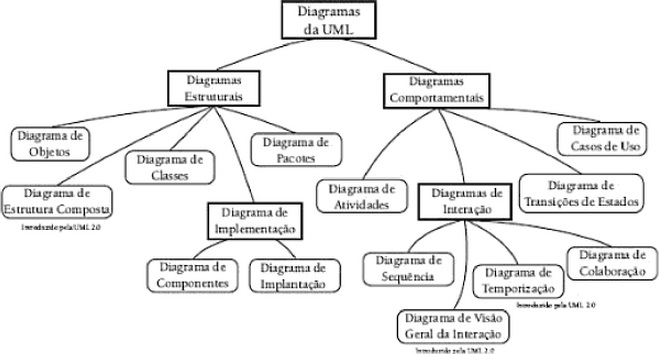
\includegraphics[scale=0.8]{./imagens/1_q_teorico/qt4.png}}
				\caption[Principais Diagramas definidos pela UML.]{Diagramas definidos pela
				UML. \textbf{Fonte:}\citeonline{2015principios}}
				\label{fig:qt4}
		\end{figure}
		
		\pagebreak
		\par A linguagem de modelagem UML não é um processo rígido e permite uma
		adequação de acordo com a situação do projeto em que é aplicada. Por permitir
		essa flexibilidade e prover suporte adequado para determinados casos de um
		projeto, é que a linguagem de modelagem UML será usada na modelagem dos
		\textit{softwares} propostos nos objetivo s dessa pesquisa.

	
	\subsection{Processos de \textit{Software}}
	
	
	\par Segundo \citeonline[p.52]{pressman2011}, um processo de \textit{software} é
“uma metodologia para as atividades, ações e tarefas necessárias para
desenvolver um \textit{software} de alta qualidade”.

	\par Para \citeonline{sommerville2003}, não existe um processo ideal, pois isso
dependerá de cada projeto, possibilitando cada qual implementar algum modelo já
existente. Contudo \citeonline{pressman2011} afirma que uma metodologia
genérica tem cinco passos:
	\begin{itemize}
	  
	  \item Comunicação - Antes de iniciar os trabalhos técnicos deve-se entender
	  os objetivos do sistema e levantar requisitos para o bom funcionamento do
	  \textit{software}.
	  
	  \item Planejamento - Cria um plano de projeto, que conterá as tarefas a
	  serem seguidas, riscos prováveis e recursos necessários.
	  
	  \item Modelagem - Esboça o sistema para que se tenha uma ideia de como ele
	  deverá ficar e como encontrar a melhor solução para desenvolve-lo.
	  
	  \item Construção - É a etapa de desenvolvimento e teste.
	  
	  \item Emprego - O \textit{software} pronto em sua totalidade ou parcialmente
	  é implantado no cliente e este retorna o seu \textit{feedback}.
	 
	 \end{itemize}
	 
	 \par Dessa forma, normalmente qualquer um dos modelos (ciclo de vida clássico,
evolutivo ou espiral) utilizaram os princípios das metodologias acima citadas.
	
\section{\textbf{Google Cloud 	Messaging}}

	\par Para que os alunos sejam notificados quando houver alguma mudança no
portal do aluno será utilizada uma API oferecida pela \textit{Google}
denominada \textit{Google Cloud Messaging} ou simplesmente
GCM\footnote{\textit{Google Cloud Messaging}}, um recurso que tem por objetivo
notificar as aplicações Android. Segundo \citeonline{leal2014} ele permite que
aplicações servidoras possam enviar pequenas mensagens de até 4
KB\footnote{\textit{Kilobytes}} para os aplicativos moveis, sem que esta
necessite estar em execução, pois o sistema operacional envia mensagens em
\textit{broadcast}, dessa forma a aplicação pode tratar as mensagens como bem
preferir.
	\par De acordo com \citeonline{leal2014} para o bom funcionamento do recurso
apresentado, são necessários os seguintes componentes:

\begin{itemize}
	
	\item \textit{Sender ID\footnote{Identity}} – É o identificador do projeto.
	Será utilizado pelo servidores da \textit{Google} para identificar a aplicação
	que envia a mensagem.
	
	\item \textit{Application ID} – É o identificador da aplicação Android. O
	identificador é o nome do pacote do projeto que consta no AndroidManifest.xml.
	
	\item \textit{Registration ID} – É o identificador gerado pelo servidor GCM
	quando aplicação Android se conecta a ele. Deve ser enviado também a aplicação
	servidora.
	
	\item \textit{Sender Auth Token} – É uma chave que é incluída no cabeçalho
	quando a mensagem é enviada da aplicação servidora para o GCM. Essa chave é
	para que a API da Google possa enviar as mensagens para o aplicativo correto.

\end{itemize}

	\par De acordo com os componentes acima citados, quando uma aplicação servidora
enviar uma mensagem para o aplicativo Android, na verdade está enviando para o
servidor GCM que será encarregado de enviar a mensagem para a aplicação mobile.
\section{\textit{Jersey}}
\section{\textit{Hibernate}}